\section{Practical application}
\label{sec:pract-appl}

\includegraphics[width=0.3in]{baustelle} better introduction

The goverment debt market is the usual data source if we want to estimate a zero-coupon yield curve for a country. Government bonds are usually the most liquid, and can be considered default-free, provided the issuing country has a good rating. We demonstrate the usage of our package with a dataset of European government bonds. Of course, a zero-coupon yield curve can also be estimated for coporate bonds. In that case, it would is interesting to compare the curve to a risk-free one and calculate the spread.


\subsection{Nelson/Siegel}

\begin{Schunk}
\begin{Sinput}
> library(termstrc)
\end{Sinput}
\end{Schunk}

\begin{Schunk}
\begin{Sinput}
> data(eurobonds)
> group <- c("GERMANY", "AUSTRIA", "ITALY")
> bonddata <- eurobonds
> matrange <- c(2, 12)
> method <- "Nelson/Siegel"
> fit <- "prices"
> weights <- "none"
> control <- list(eval.max = 1e+05)
> b <- matrix(c(0, 0, 0, 1, 0, 0, 0, 1, 0, 0, 0, 1), nrow = 3, 
+     ncol = 4, byrow = TRUE)
> rownames(b) <- group
> colnames(b) <- c("beta0", "beta1", "beta2", "tau1")
\end{Sinput}
\end{Schunk}

\begin{Schunk}
\begin{Sinput}
> x <- nelson_estim(group, bonddata, matrange, method, fit, weights, 
+     startparam = b, control)
> print(x)
\end{Sinput}
\begin{Soutput}
---------------------------------------------------
Parameters for Nelson/Siegel, Svensson estimation:

Method: Nelson/Siegel 
Fitted: prices 
Weights: none 

---------------------------------------------------

             GERMANY     AUSTRIA       ITALY
beta_0  0.0418991850  0.04167176  0.04645068
beta_1 -0.0190504299 -0.01716246 -0.02012130
beta_2 -0.0001155352 -0.01451567 -0.02134967
tau_1   3.9893303512  2.11920557  2.39845119

---------------------------------------------------
Parameters for Nelson/Siegel, Svensson estimation:

Method: Nelson/Siegel 
Fitted: prices 
Weights: none 

---------------------------------------------------

             GERMANY     AUSTRIA       ITALY
beta_0  0.0418991850  0.04167176  0.04645068
beta_1 -0.0190504299 -0.01716246 -0.02012130
beta_2 -0.0001155352 -0.01451567 -0.02134967
tau_1   3.9893303512  2.11920557  2.39845119
\end{Soutput}
\end{Schunk}

\begin{Schunk}
\begin{Sinput}
> summary(x)
\end{Sinput}
\begin{Soutput}
---------------------------------------------------
Goodness of fit:
---------------------------------------------------

                  GERMANY      AUSTRIA        ITALY
RMSE-Prices  1.059285e-01 2.868050e-02 0.0790745094
AABSE-Prices 6.157349e-02 2.000662e-02 0.0561561019
RMSE-Yields  1.324394e-04 4.051508e-05 0.0001240929
AABSE-Yields 8.941224e-05 2.994120e-05 0.0001016403


---------------------------------------------------
Convergence information:
---------------------------------------------------

        Convergence ()  
GERMANY "no convergence"
AUSTRIA "converged"     
ITALY   "converged"     

        Solver message                                   
GERMANY "iteration limit reached without convergence (9)"
AUSTRIA "relative convergence (4)"                       
ITALY   "relative convergence (4)"                       
\end{Soutput}
\end{Schunk}

\begin{center}
\begin{Schunk}
\begin{Sinput}
> par(mfrow = c(3, 2), cex = 0.55)
> plot(x)
\end{Sinput}
\end{Schunk}
\includegraphics{example-005}
\end{center}

\subsection{Cubic Splines}

\begin{Schunk}
\begin{Sinput}
> data(eurobonds)
> group <- c("GERMANY", "AUSTRIA", "ITALY")
> bonddata <- eurobonds
> matrange <- "all"
\end{Sinput}
\end{Schunk}

\begin{Schunk}
\begin{Sinput}
> x <- splines_estim(group, bonddata, matrange)
> print(x)
\end{Sinput}
\begin{Soutput}
---------------------------------------------------
Parameters for Cubic splines estimation:

[1] "GERMANY:"
      alpha 1       alpha 2       alpha 3       alpha 4       alpha 5 
-0.0031562638 -0.0001804021  0.0008893256  0.0009869789 -0.0235685086 

[1] "AUSTRIA:"
      alpha 1       alpha 2       alpha 3       alpha 4 
-0.0030226383  0.0007101622  0.0010939255 -0.0234513152 

[1] "ITALY:"
      alpha 1       alpha 2       alpha 3       alpha 4       alpha 5 
-1.319834e-03 -2.612472e-03 -3.871354e-05  1.264864e-03  6.204093e-04 
      alpha 6 
-2.481481e-02 
\end{Soutput}
\end{Schunk}


\begin{Schunk}
\begin{Sinput}
> summary(x)
\end{Sinput}
\begin{Soutput}
---------------------------------------------------
Goodness of fit:
---------------------------------------------------

                  GERMANY      AUSTRIA        ITALY
RMSE-Prices  1.818950e+01 1.386148e+01 2.283539e+01
AABSE-Prices 1.406844e+01 8.328159e+00 1.536100e+01
RMSE-Yields  1.224657e-04 1.114989e-04 1.499874e-04
AABSE-Yields 8.282076e-05 8.727466e-05 1.155357e-04

---------------------------------------------------
Summary statistics for the fitted models:
---------------------------------------------------

$GERMANY

Call:
lm(formula = -Y[[k]] ~ X[[k]] - 1)

Residuals:
      Min        1Q    Median        3Q       Max 
-0.133728 -0.043399 -0.009263  0.019054  0.337135 

Coefficients:
          Estimate Std. Error t value Pr(>|t|)    
alpha 1 -3.156e-03  4.765e-04  -6.623 7.51e-07 ***
alpha 2 -1.804e-04  1.572e-04  -1.148    0.262    
alpha 3  8.893e-04  4.782e-05  18.598 9.25e-16 ***
alpha 4  9.870e-04  6.148e-05  16.053 2.45e-14 ***
alpha 5 -2.357e-02  5.786e-04 -40.734  < 2e-16 ***
---
Signif. codes:  0 ‘***’ 0.001 ‘**’ 0.01 ‘*’ 0.05 ‘.’ 0.1 ‘ ’ 1 

Residual standard error: 0.1084 on 24 degrees of freedom
Multiple R-Squared:     1,	Adjusted R-squared:     1 
F-statistic: 1.693e+06 on 5 and 24 DF,  p-value: < 2.2e-16 


$AUSTRIA

Call:
lm(formula = -Y[[k]] ~ X[[k]] - 1)

Residuals:
       Min         1Q     Median         3Q        Max 
-0.0806338 -0.0430618  0.0006852  0.0263651  0.1077566 

Coefficients:
          Estimate Std. Error t value Pr(>|t|)    
alpha 1 -3.023e-03  1.274e-04  -23.72 4.03e-10 ***
alpha 2  7.102e-04  4.795e-05   14.81 3.95e-08 ***
alpha 3  1.094e-03  8.459e-05   12.93 1.44e-07 ***
alpha 4 -2.345e-02  2.255e-04 -104.01  < 2e-16 ***
---
Signif. codes:  0 ‘***’ 0.001 ‘**’ 0.01 ‘*’ 0.05 ‘.’ 0.1 ‘ ’ 1 

Residual standard error: 0.05827 on 10 degrees of freedom
Multiple R-Squared:     1,	Adjusted R-squared:     1 
F-statistic: 1.479e+06 on 4 and 10 DF,  p-value: < 2.2e-16 


$ITALY

Call:
lm(formula = -Y[[k]] ~ X[[k]] - 1)

Residuals:
      Min        1Q    Median        3Q       Max 
-0.268791 -0.051542 -0.003029  0.056274  0.162438 

Coefficients:
          Estimate Std. Error t value Pr(>|t|)    
alpha 1 -1.320e-03  1.827e-03  -0.722    0.476    
alpha 2 -2.612e-03  4.548e-04  -5.745 2.85e-06 ***
alpha 3 -3.871e-05  9.279e-05  -0.417    0.679    
alpha 4  1.265e-03  4.061e-05  31.149  < 2e-16 ***
alpha 5  6.204e-04  6.910e-05   8.978 5.29e-10 ***
alpha 6 -2.481e-02  1.180e-03 -21.029  < 2e-16 ***
---
Signif. codes:  0 ‘***’ 0.001 ‘**’ 0.01 ‘*’ 0.05 ‘.’ 0.1 ‘ ’ 1 

Residual standard error: 0.1005 on 30 degrees of freedom
Multiple R-Squared:     1,	Adjusted R-squared:     1 
F-statistic: 2.049e+06 on 6 and 30 DF,  p-value: < 2.2e-16 
\end{Soutput}
\end{Schunk}

\begin{center}
\begin{Schunk}
\begin{Sinput}
> par(mfrow = c(3, 2), cex = 0.55)
> plot(x)
\end{Sinput}
\end{Schunk}
\includegraphics{example-009}
\end{center}




\subsection{Dynamic estimation}

In the following, we provide results for a dynamic estimation of the zero-coupon yield curve for the time between November 30, 2007 and February 1, 2008. We used the \cite{Svensson1994} method, together with duration weights and minimization of the price errors. Fig. \ref{fig:3dplot} shows how the estimated French yield curves.

\begin{figure}[htb]
  \begin{center}
  \caption{Zero-coupon yield curves in France}
  \label{fig:3dplot}
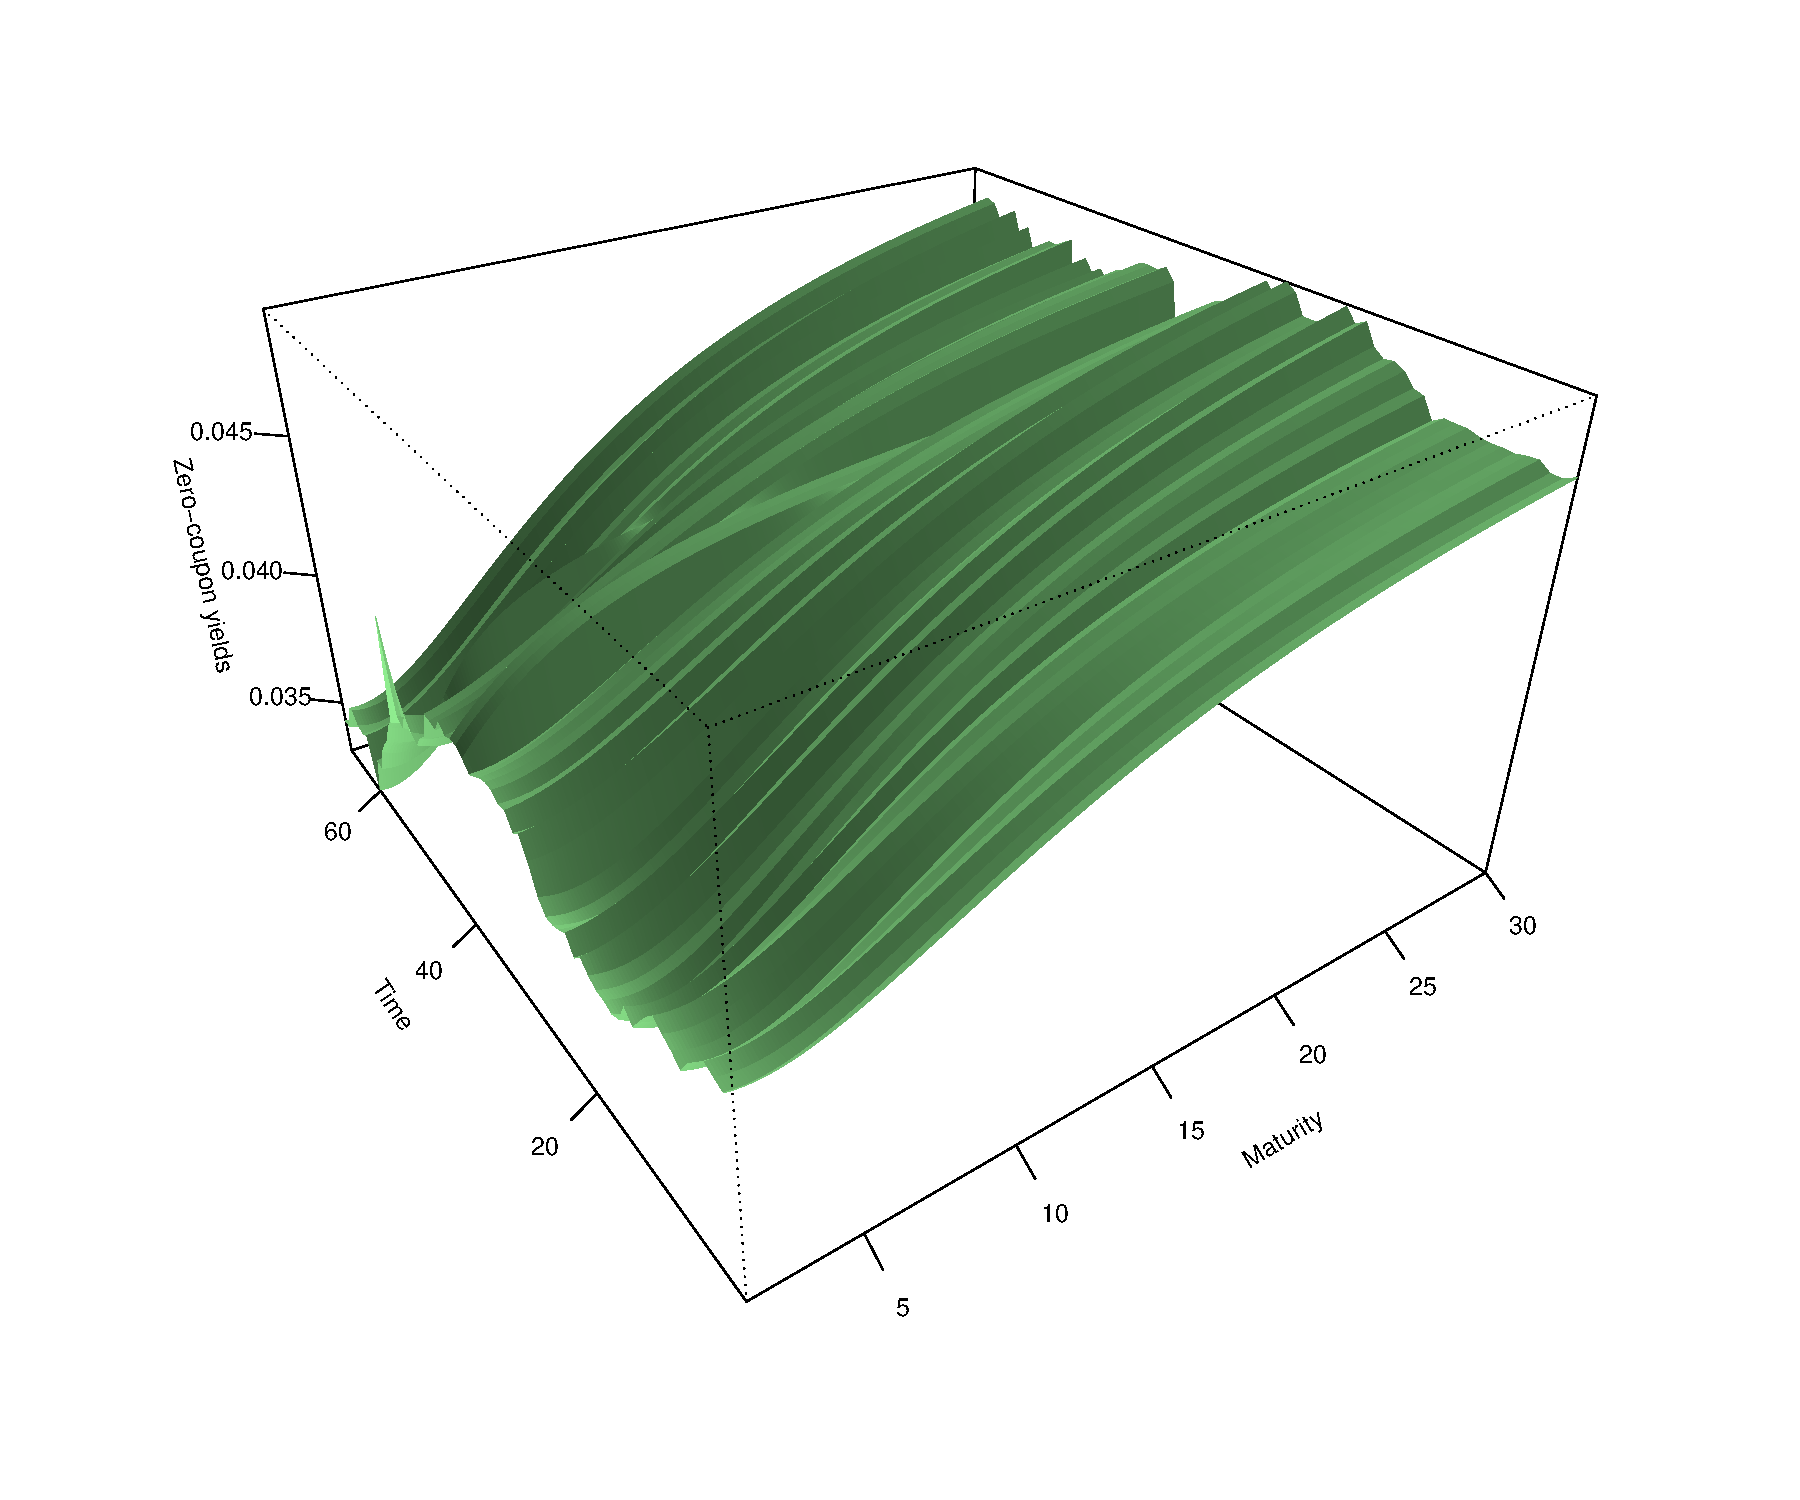
\includegraphics[width=0.7\textwidth]{3dplot}
\end{center}
\end{figure}

Fig. \ref{fig:paramdevel} shows how the parameters evolve over time. To speed up the estimation and ensure the algorithm stays in a global minimum, the estimated parameters from the previous period were used as start parameters for the next one.

\begin{figure}[htb]
  \begin{center}
  \caption{Estimated parameters}
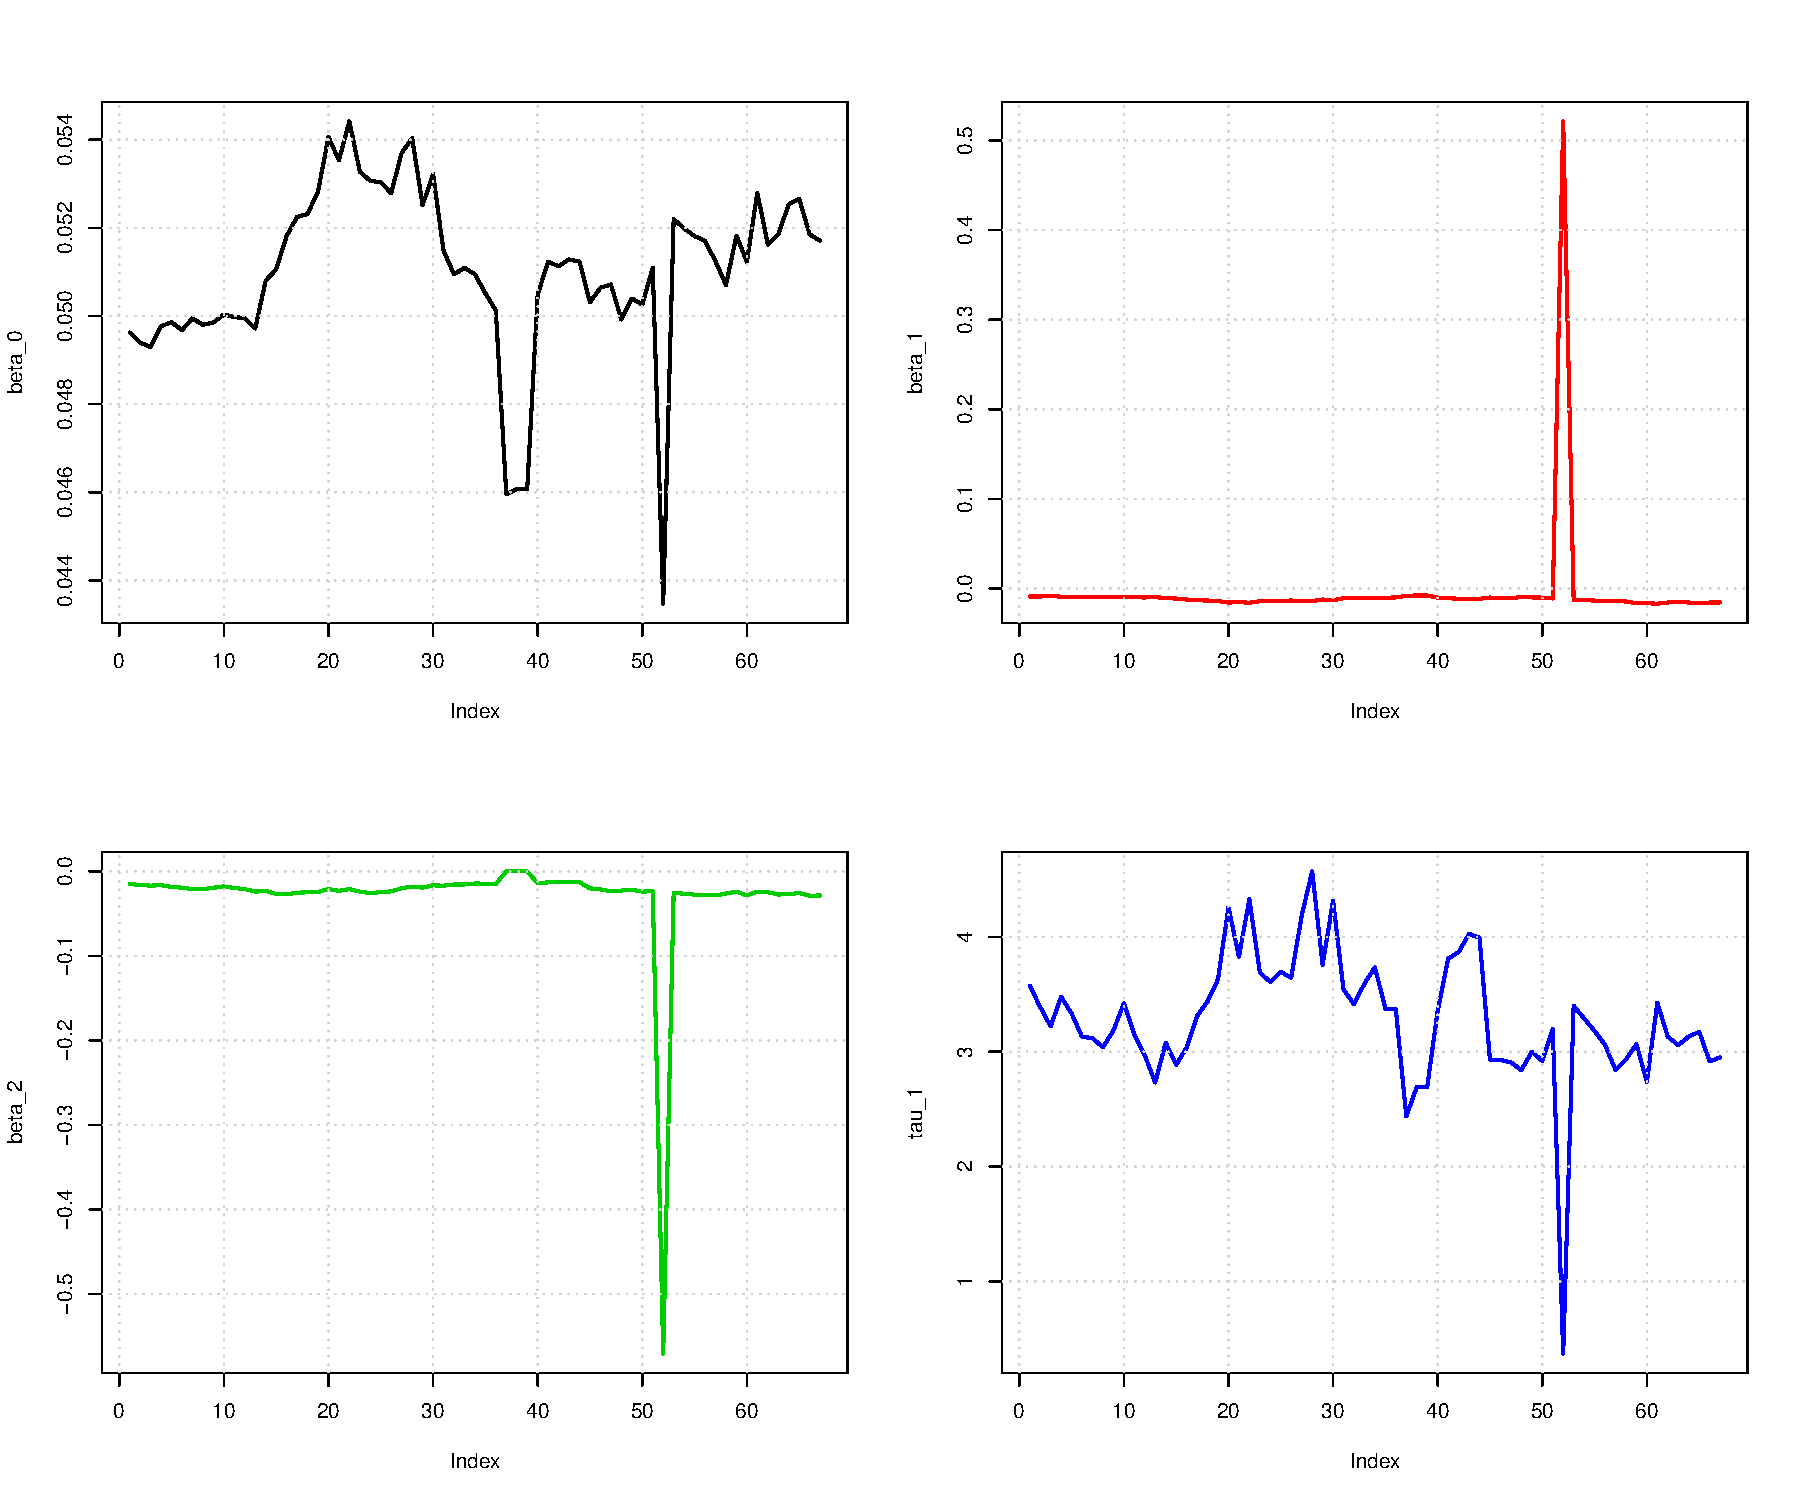
\includegraphics[width=0.8\textwidth]{paramdevel}
\label{fig:paramdevel}
\end{center}
\end{figure}



%%% Local Variables: 
%%% mode: latex
%%% TeX-master: "jss-termstrc"
%%% End: 